\documentclass[rapport.tex]{subfiles}

\begin{document}
\section{Analyse}
	\subsection{Indledning}
	Formålet med analysedelen af projektet var at få en indledende indsigt i emnet. Det indebar at få skabt et overblik over hvad der skulle laves, hvorfor det skulle laves, og hvilke krav der er til de ting som skulle laves. Størstedelen af tiden i denne fase af projektet blev brugt på at forstå den udleverede kode. En væsentlig del af tiden blev også brugt på at undersøge hvordan ændringer kunne påvirke resultater og performance, samt hvilke steder disse ændringer bedst kunne foretages. Det er også vigtigt at nævne at det der bliver gennemgået i dette afsnit overvejende er koncepter eller teori, med tilhørende eksempler rettet mod at fremme forståelsen. Konkret design og implementering vil blive gennemgået senere, i design og implementeringsdelene af rapporten.
	
	\subsection{Systemoversigt}
	
	Blokdiagram: Userskærm, testskærm, IR-LED, kamera.
	Blokdiagram2: Overordnet blokdiagram over software. (Figur 2, geometric approach to eyetracking)
	
	Billede af opstilling.
	
	
	
	
	Dette er opstillingen som projektet tager udgangspunkt i. Argumentationen for valget af denne opstilling kan ses i indledningen til projektet (Ref indledning).
	
	\subsection{Funktionalitetskrav}
	
		I løbet af analysen blev der løbende fremstillet en kravspecifikation, i samarbejde med projektudbyderen. En del af denne kravspecifikation bestod af Use Cases, en række situationer man kunne forestille sig ville opstå, når man anvender systemet. Formålet med dem er at dække en række situationer der kunne opstå, hvad enten systemet gør som tiltænkt eller hvis det af forskellige årsager fejler. Dette gør det lettere at designe et konkret system, idet man har en lang række hændelser som systemet skal kunne håndtere. I rapporten er der valgt kun at vise en enkelt Use Case, de resterende Use Cases kan ses i dokumentet kravspecifikation.pdf (Se appendiks). 
	
		\subsubsection{Use case eksempel - Start måling}
		I figur \ref{fig:UseCase3} ses et eksempel på en use case for systemet. Denne use case er skrevet ud fra kravet om at man skal kunne påbegynde real-time eye-tracking fra en knap i det grafiske bruger-interface.
		
		\begin{figure}
		\caption{Use case 3}
		\label{fig:UseCase3}
		\begin{tabular}{|l|p{7.7cm}|}
			\hline \textbf{Sektion} 	& \textbf{Kommentar} \\ 
			\hline Mål  & Programmet påbegynder real-time eye-tracking \\ 
			\hline Initiering  & Initieres af aktøren \textit{bruger} \\ 
			\hline Aktører & Aktøren \textit{bruger} og aktøren \textit{kamera} \\ 
			\hline Antal samtidige forekomster & 1 \\ 
			\hline Startbetingelser & Computerprogrammet skal være opstartet, \textit{kamera} skal være tændt, programmet skal være kalibreret. \\ 
			\hline Slutresultat – succes & Programmet har påbegyndt real-time eye-tracking\\ 
			\hline Slutresultat – undtagelse & Programmet alarmerer \textit{bruger} at der ikke er foretaget kalibrering \\ 
			\hline Normal forløb & \begin{enumerate}
				\item \textit{Bruger} klikker på knappen ”Start”.
				\item Programmet starter ny måling.
				\item Visuel feedback på GUI viser at måling er i gang.
			\end{enumerate} \\  
			\hline Undtagelsesforløb & Programmet kan ikke starte ny måling. Programmet melder
			at kalibrering ikke er foretaget.\\
			\hline 
		\end{tabular}
		\end{figure}
		
	\subsection{Overvejelser, Funktionelle krav}	
	
	\subsubsection{Real-time eye-tracking}
	Dette krav er stillet af udbyderen af projektet, og kan betragtes som et af de mest fundamentale krav i projektet. Projektet udspringer fra et tidligere projekt, hvor billedbehandlingen af kameradata foregik offline. Det skal optimeres i en tilstrækkelig grad til at kunne køre i realtime i stedet for, med en framerate på 100 billeder per sekund.
	
	\subsubsection{Kalibrering}
	For at systemet kan fungere korrekt skal der først foretages en kalibrering. Målinger kan foretages uden kalibrering, men det vil ikke være muligt at oversætte de resulterende data til et sæt skærmkoordinater. Denne kalibrering er derfor essentiel for systemet.
	
	\subsubsection{Output}
	Resultater fra målinger skal gemmes i en log-fil tilgængelig til brugeren. Dette krav stammer fra et ønske fra udbyder om at have adgang til data efter behandling. I
	design-delen af rapporten kan ses en protokol, der beskriver hvordan data skal gemmes i log-filen. 
	
	
	
	De resterende funktionelle krav er blevet uddybet ved hjælp af Use Cases -REF-.
	
	
	\subsection{Overvejelser, Ikke-funktionelle krav}
	
	\subsubsection{Fejlmargin}
	
	
	
	\subsubsection{Real-time}
	
	
	
	\subsubsection{Modularisering}
	essentielt for projektet. Programmet skal skrives som en API (Application Programming Interface), altså et software-interface til anden software. Denne API skal designes således at bruger-interfacet, håndteringen af diverse filer, logning af data, kommunikation med hardware og så videre, kan implementeres som sit eget stykke software. Denne software kan så være basis for algoritmer der overholder API'ens regler. 
	rænseflade, tilstrækkelig
	funktionalitet til at dække formodede behov, samt et design der gør det let at udvide
	applikationen på et senere tidspunkt.
	
	\subsubsection{Kodesprog}
	Det er blevet aftalt med projektudbyder at prototypen skal udarbejdes med en C++ backend "Algoritmer" og Python frontend "Bruger interface".
	C++ er valgt som backend fordi det er et relativt hurtigt kodesprog, og fordi gruppen har tidligere erfaring
	med C++. Python blev foreslået til gruppen af projektvejleder, og idet Python har udvidelser der er opbygget
	i C/C++ "OpenCV og Numpy" var det en oplagt mulighed at anvende Python til front end delen af prototypen.
	                           
	\subsection{Starburst-algoritmen}
	I det følgende vil algoritmen som projektet tager udgangspunkt i blive gennemgået.
	
	Bemærk at der udelukkende beskrives hvad Starburst-algoritmen gør, og at der i følgende afsnit IKKE bliver beskrevet hvordan andre problematikker (For eksempel lokalisering af øjne og lokalisering af pupilmidtpunkt) bliver løst. Håndteringen af disse vil dog blive gennemgået i implementeringsdelen af rapporten.
	
	Algoritmen kan opdeles i følgende punkter "ref starburst":
	
	Input: Billede.
	Output: Gaze vektor
	Procedure:
	Detekter hornhinde reflektioner.
	Lokaliser hornhinde reflektioner.
	Fjern hornhinde reflektioner.
	Iterativ detektion af pupil kantpunkter.
	RANSAC "Random Sample Consensus" for at finde en passende ellipse.
	Anvend kalibrering til at omsætte vektoren imellem midten af hornhinde reflektionerne og midten af pupillen, til skærmkoordinater i pixels.
	
	----------------------
	
	\begin{figure}
	\centering
	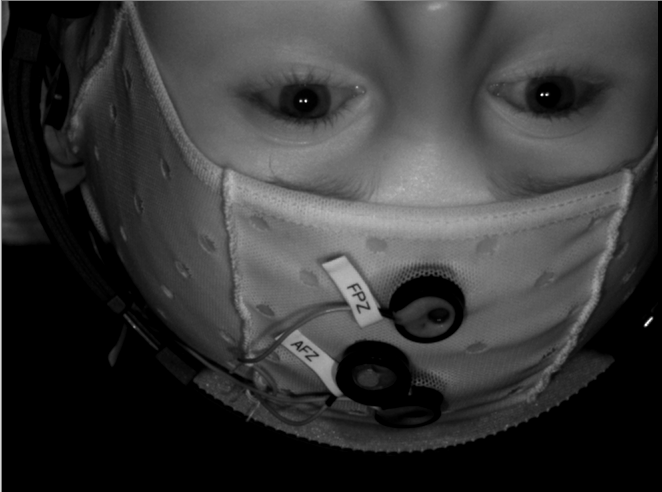
\includegraphics[width=0.4\linewidth]{Billeder/InitialImage.png}
	\caption{Enkelt billede fra video optagelse}
	\label{fig:InitialImage}
	\end{figure}
	
	Gennemgangen tager udgangspunkt i det ovenstående billede, som er det første billede i videoen "Derp""Kan findes på CD'en, filsti". Det første der bliver gjort er at få lavet et såkaldt "Region of Interest" i billedet, en afgrænsning af billedet til det område der er relevant for algoritmen, altså øjnene. Dette gøres for at spare på ressourcer under behandlingen af billedet, da der er væsentligt færre pixels i forhold til at bruge hele billedet i alle udregninger. Der findes flere forskellige metoder til at opnå dette, eksempelvist kunne man inden opstart manuelt markere et område som algoritmen skal fokusere på i det første billede, og derefter bruge det tidligere billede som udgangspunkt i de efterfølgende billeder.
	
	\begin{figure}
	\centering
	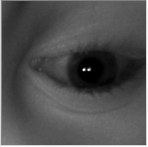
\includegraphics[width=0.4\linewidth]{Billeder/CroppedEye.png}
	\caption{Udsnit af øje}
	\label{fig:CroppedEye}
	\end{figure}
	
	Når det relevante område af billedet er fundet, kan Starburst algoritmen anvendes. Man kan dog med fordel forsøge at øge kontrasten i billedet, således at differensen imellem pupil og iris øges. Dette gør algoritmen mere robust, da der vil være en mere klar adskillelse af overgangen fra pupil til iris. Årsagen til at dette gør algoritmen mere robust vil være lettere at forstå efter gennemgangen af detektionen af pupilkantpunkter.
	
	\begin{figure}
	\centering
	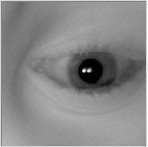
\includegraphics[width=0.4\linewidth]{Billeder/CroppedEye,PostBrightness.png}
	\caption{Efter øgning af kontrast og lysstyrke}
	\label{fig:CroppedEye,PostBrightness}
	\end{figure}
	
	Efterfølgende skal reflektionerne i øjet lokaliseres og fjernes. Alternativt kan man også blot gemme områderne for reflektionerne, og tage højde for dem i sin algoritme i stedet.
	
	\begin{figure}
	\centering
	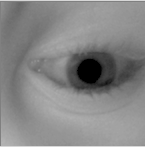
\includegraphics[width=0.4\linewidth]{Billeder/CroppedEye,Reflectionremoved.png}
	\caption{Reflektioner fjernet}
	\label{fig:CroppedEye,Reflectionremoved}
	\end{figure}
	
	Efter fjernelsen af reflektionerne, er det tid til den del af algoritmen som den har fået sit navn fra. Fra et estimeret midtpunkt af pupillen"ref" bliver en række "stråler" sendt ud imod kanten af billedet, og når de rammer en tilpas kraftig ændring i intensitet stopper de, og det antages at de har ramt en overgang fra pupil til iris.
		
	\begin{figure}
	\raggedright
	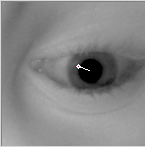
\includegraphics[width=0.4\linewidth]{Billeder/Starburst,Firstsingle.png}
	\caption{Starburst, første iteration (Enkelt stråle)}
	\label{fig:Starburst,Firstsingle}
	\end{figure}	
		
	\begin{figure}
	\raggedleft
	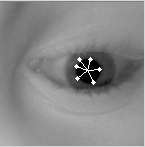
\includegraphics[width=0.4\linewidth]{Billeder/Starburst,First.png}
	\caption{Starburst, første iteration (Resterende stråler)}
	\label{fig:Starburst,First}
	\end{figure}
	
	Resultatet af dette er en række punkter som, ifølge hensigten, ligger på kanten af pupillen. Idet der er en risiko for at algoritmen finder punkter som ikke ligger på pupilkanten, gentages Starburst, med hvert fundet punkt som et nyt midtpunkt. Derudover tilpasses vinklerne som strålerne kan sendes ud i, sådan at de søger ind imod det oprindelige startpunkt, + / - et forskelligt antal grader. Dermed får man en række stråler, der oftest vil ramme pupilkanten, og dermed skabe flere brugbare punkter til næste del af algoritmen.
	
	\begin{figure}
	\centering
	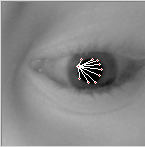
\includegraphics[width=0.4\linewidth]{Billeder/Starburst,Secondsingle.png}
	\caption{Starburst, anden iteration (Et startpunkt)}
	\label{fig:Starburst,Secondsingle}
	\end{figure}
	
	\begin{figure}
	\centering
	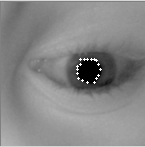
\includegraphics[width=0.4\linewidth]{Billeder/Starburst,Second.png}
	\caption{Starburst, anden iteration (Alle Punkter)}
	\label{fig:Starburst,Second}
	\end{figure}
		
	Ovenstående billede til venstre illustrerer hvordan strålerne sendes ud fra et tidligere punkt, og billedet til højre viser det endelige resultat af Starburst algoritmen. Ud fra disse punkter kan en ellipse så tilpasses, ved hjælp af RANSAC (Random Sample Consensus). RANSAC fungerer ved at udvælge en vis mængde af de fundne punkter (I vores tilfælde fem), og derefter undersøge hvor godt punkterne passer ind i en model (En model for en ellipse i denne algoritme).
			
	\begin{figure}
	\centering
	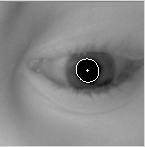
\includegraphics[width=0.4\linewidth]{Billeder/Starburst,Ellipse.png}
	\caption{Resulterende ellipse}
	\label{fig:Starburst,Ellipse}
	\end{figure}
	
	Efter RANSAC har kørt, ender man med et sæt punkter som kan danne en ellipse. Midten af denne ellipse skulle så gerne være midten af pupillen, og med det punkt, samt midtpunktet imellem de to reflektioner, kan man finde gaze  vektoren.
	
	\begin{figure}
	\centering
	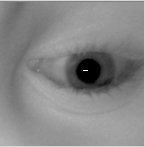
\includegraphics[width=0.4\linewidth]{Billeder/Starburst,Gaze.png}
	\caption{Resulterende gaze vektor}
	\label{fig:Starburst,Gaze}
	\end{figure}
	
	Bemærk at gaze vektoren i sig selv ikke kan fortælle nøjagtigt hvor en person ser hen. Dertil skal man have kalibreret systemet først, ved at gennemgå kalibreringsrutinen som nævnt i "ref". Udfra dette kan man så lave en homografisk mapning ved hjælp af interpolering, som i sidste ende kan bruges til at omsætte gaze vektoren til et sæt skærmkoordinater.
	
	\subsection{OpenEyes og Siboska}
	Tidligt i projektforløbet blev der udleveret kildekode til gruppen, kildekode som prototypen overvejende er inspireret af "Siboskas kode". Derudover er der også kildekoden som Siboska implementeringen har taget sit udspring i. Et eksempel på væsentlige forskelle og egenskaber vil kort blive gennemgået, og resterende eksempler kan findes i analyseafsnittet i dokumentationen "Ref". En sammenligning af gruppens implementering og disse implementeringer vil blive lavet i implementeringsdelen af rapporten.
	
	Idet der ville være behov for en uvis mængde tid for at få OpenEyes koden op og køre, blev det valgt kun at bruge det kode som mulig inspirationskilde, og derfor er alt simulering foregået i Matlab med Siboska koden.
	
	\subsection{Algoritme Oversigt}
	
	Matlabprofiler - procentvis brug af hver del af algoritmen.
	Bemærk at procestiden er opgivet som procentdel af samlet procestid, og at værdierne kun omfatter processen selv, og ikke medregner den tid der bruges på metoder der kaldes undervejs. Procestiden for disse metodekald står ud for de enkelte metoder i stedet.
	
	\begin{figure}[h]
		\centering
		\includegraphics[width=0.7\linewidth]{../Algoritmediagram.png}
		\caption[Systemdiagram]{Systemdiagram for Real-time eye-tracking}
		\label{fig:Systemdiagram}
	\end{figure}
	
	Samlet tid, antal frames, indsæt profiler udsnit, forklar.
	Forklar nedenstående.
	
	\subsubsection{Calculate pupil and gaze}
	
	Main funktion - 0.17%
	
	\subsubsection{Locate corneal reflection}
	
	Finder reflektionspunker - 0.3%
	
	\subsubsection{Starburst pupil contour detection}
	
	Starburst algoritme - 0.63%
	
	\subsubsection{Locate Edge Points}
	
	Find pupil kant punkter - 44.71%
	
	\subsubsection{Fit ellipse ransac}
	
	Tilpas en ellipse til punkterne - 11.7%
	
	\subsection{Fokuspunkter}
	I det følgende underafsnit vil der kort blive beskrevet hvilke dele af koden der blev fokuseret på. Begrundelsen for fokus er baseret på antal gange rutinen bliver kørt, samt hvor lang tid det tager for hele processen at blive færdig.
	
	\subsubsection{Kantdetektion}
	Den mest tidskrævende del af algoritmen er selve starburst-delen, altså den del hvor pupilkantpunkter findes. Udover / i stedet for at optimere koden, er der også mulighed for at justere variabler for at få processen til at tage kortere tid. Dette kan i nogle tilfælde gøres uden problemer"ref RANSAC", og i andre tilfælde på bekostning af resultaternes nøjagtighed/præcision, eller systemets overordnede stabilitet. Der vil altså formentligt være behov for en balancering af performance overfor kvalitet i nogle tilfælde. Denne balancering vil foregå iterativt i løbet af implementeringsfasen af projektet.
	
	\subsubsection{Ellipse Tilpasning}
	Den næstmest tidskrævende del af algoritmen er ellipsetilpasningen. Her vil det igen være muligt at justere på variabler, for at balancere performance og kvalitet. Derudover skal der ses nærmere på undtagelsestilstande hvor algoritmen gentages mange gange, RANSAC iterations = 10000. Hvis disse undtagelsestilstande opsluger meget tid og sker ofte, kunne det have en markant effekt på performance for systemet.
	
	\subsubsection{Kegleparametre til Ellipseparametre}
	En mindre betydelig, men dog stadig mærkbar del af algoritmen er den del som oversætter kegleparametre til ellipseparametre. Da denne del af algoritmen kun udgør omkring 6 procent af den samlede procestid, er denne blot nævnt som en mulig kandidat for optimering hvis de primære dele begynder at være sammenlignelige i procestid. 
	
	\subsubsection{Kamera Input}
	En sidste ting der med fordel kan fokuseres på at forbedre er indlæsning af data fra kameraet. Idet der ikke sker meget kompression bør det meste af arbejdet bestå af overførsler i harddisken, men hvis det viser sig at være for tungt kan vi forsøge at gøre noget.
	
	
	 hvilket også indebærer processeringstid for de enkelte subrutiner. I forlængelse af dette vil begrundelserne for krav der har med algoritmen at gøre også blive givet i en relevant kontekst.
	I det følgende vil simuleringer i forbindelse med starburst algoritmen blive gennemgået. Disse simuleringer er blevet udført i et forsøg på at danne en bedre indsigt i sammenhængen imellem performance og resultater. Idet en overgang til en anden platform end MATlab formentligt ikke forøger performance tilstrækkeligt, skal der i stedet undersøges hvorvidt det er muligt at tilpasse forskellige variabler til at opnå en kortere processeringstid, alt imens resultaterne forbliver gode.
	
	\subsection{Simulering}
	
	Simuleringerne er foretaget med det kode og videodata som Daniel Sibozka har udleveret til gruppen. I det første afsnit vises resultaterne, og i andet afsnit beskrives hvilke ændringer af variabler der afprøves, og derefter vises resultaterne af disse ændringer.
	
	\subsubsection{Extract gaze vector from video}
	
	Processeringstid, CPU = 2.4 GHz
	
	Figur over resultater.
	
	\subsubsection{Variabel Ændringer}
	
	Antal Rays
	Antal RANSAC iterationer
	
	
	\subsubsection{Resultater}
	
	Figur 
	\subsection{Diskussion}
		
\end{document}